\begin{pastexam}[label={px:df3-096-ds-03}]{地方三等資訊處理 96 年 第三題}
（申論；20 分）

解釋下列名詞並舉例說明：（每小題 5 分，共 20 分）
\begin{itemize}[leftmargin=2em, labelsep=0.3em, itemsep=1pt]
\item[㈠] 優先權佇列（priority queue）
\item[㈡] 堆積（heap）
\item[㈢] 二元搜尋樹（binary search tree）
\item[㈣] 深度優先生成樹（depth-first spanning tree）
\end{itemize}
\end{pastexam}

\begin{pastsoln}
四個名詞分屬資結書第~8、9、21~章；前兩個是同一件事的「規格」和「實作」，所以整題放在第~8~章。
每個名詞先給定義，再舉一個具體的例子。

\textbf{㈠ 優先權佇列}（資結書第~8.3~節）是一種抽象資料型態：每筆資料帶一個優先權（鍵），
支援「加入一筆」和「取出優先權最高的一筆」，有時還有「看最高的一筆」「提高某筆的優先權」。
它只規定操作的意義，不規定怎麼存。 和一般佇列的差別在取出的順序：佇列是先進先出，優先權佇列
是優先權最高的先出。

例子：作業系統排程，數字小的優先。 依序加入 (P1, 5)、(P2, 2)、(P3, 8)，取出得 P2；再加入
(P4, 1)，取出得 P4；再取出得 P1。 實作方式可以是未排序陣列（加入 $O(1)$、取出 $O(n)$）、
排序陣列（加入 $O(n)$、取出 $O(1)$）或下面的堆積（兩者都 $O(\lg n)$）。

\textbf{㈡ 堆積}（資結書第~8.1~節）：一棵完整二元樹（complete binary tree），每個節點的鍵都
不小於它子節點的鍵（最大堆積；反過來是最小堆積）。 所以根是最大值。 因為是完整二元樹，可以
不用指標，直接存在陣列 $A[1..n]$：節點 $i$ 的子節點是 $2i$、$2i+1$，父節點是
$\lfloor i/2 \rfloor$，高度 $\lfloor \lg n \rfloor$。 加入時放在最後一格往上調，取出根時把
最後一格搬到根往下調，都是 $O(\lg n)$，所以堆積是實作優先權佇列最常用的方法。

例子：$A = \langle 90, 70, 80, 20, 60, 30, 40 \rangle$ 是最大堆積：
\begin{center}
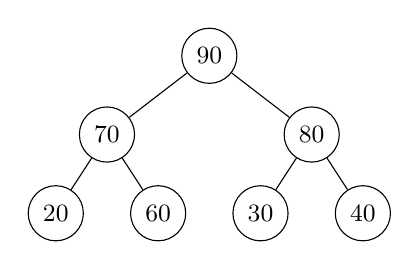
\begin{tikzpicture}[level distance=10mm,
  level 1/.style={sibling distance=26mm}, level 2/.style={sibling distance=13mm},
  every node/.style={circle, draw, minimum size=7mm, inner sep=0pt, font=\small}]
\node {90}
  child {node {70} child {node {20}} child {node {60}}}
  child {node {80} child {node {30}} child {node {40}}};
\end{tikzpicture}
\end{center}
每個父節點都 $\ge$ 子節點（$90 \ge 70, 80$；$70 \ge 20, 60$；$80 \ge 30, 40$）。 注意堆積只
規定上下，不規定左右：$70 < 80$ 在左邊也可以。

\textbf{㈢ 二元搜尋樹}（資結書第~9~章）：一棵二元樹，每個節點 $x$ 的左子樹所有鍵都 $< x$
的鍵，右子樹所有鍵都 $> x$ 的鍵（鍵不重複時）。 搜尋從根開始，比根小往左、比根大往右，
每層只比一次，搜尋、加入、刪除都是 $O(h)$，$h$ 是樹高；中序走訪會由小到大列出所有鍵
（資結書定理~9.1）。

例子：依序加入 $50, 30, 70, 20, 40, 60$：
\begin{center}
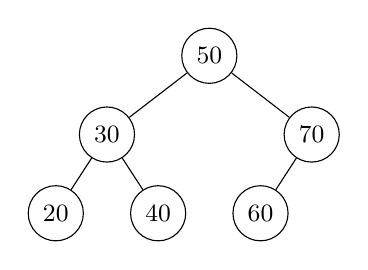
\begin{tikzpicture}[level distance=10mm,
  level 1/.style={sibling distance=26mm}, level 2/.style={sibling distance=13mm},
  every node/.style={circle, draw, minimum size=7mm, inner sep=0pt, font=\small}]
\node {50}
  child {node {30} child {node {20}} child {node {40}}}
  child {node {70} child {node {60}} child[missing]};
\end{tikzpicture}
\end{center}
找 $40$：$40 < 50$ 往左，$40 > 30$ 往右，找到，比了 $3$ 次。 中序是 $20, 30, 40, 50, 60, 70$。
和㈡的堆積比較：堆積是「上大下小」，二元搜尋樹是「左小右大」，所以堆積找最大值快，但找任意
一個鍵要 $O(n)$。

\textbf{㈣ 深度優先生成樹}（資結書第~21.4~節）：對一個連通圖做深度優先搜尋（DFS），每次從
$u$ 沿邊 $(u, v)$ 走到一個還沒拜訪過的 $v$，就把 $(u, v)$ 記下來；這些邊（共 $|V| - 1$ 條）
連起所有頂點、沒有環，形成一棵以起點為根的生成樹，稱為深度優先生成樹。 圖中其他沒用到的邊在
無向圖裡都是「後向邊」：一端是另一端的祖先（資結書定理~21.8）。 同一張圖，起點或鄰居的順序
不同，得到的樹也可能不同。

例子：下面左圖從 $1$ 開始，鄰居依編號由小到大，拜訪順序 $1, 2, 4, 3, 5$；走過的邊
$(1,2)$、$(2,4)$、$(4,3)$、$(3,5)$ 構成右邊的深度優先生成樹，$(1,3)$ 和 $(2,5)$ 是後向邊。
\begin{center}
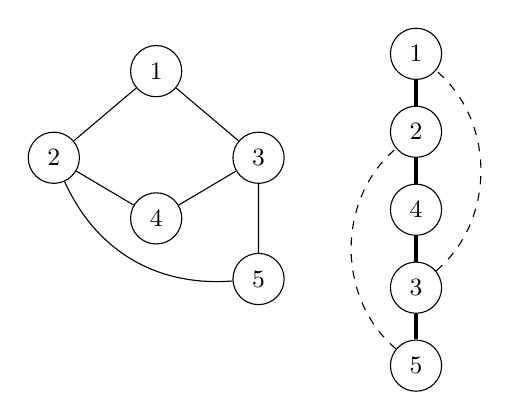
\begin{tikzpicture}[x=1.3cm, y=1.1cm,
  v/.style={circle, draw, minimum size=6.5mm, inner sep=0pt, font=\small}]
\begin{scope}
\node[v] (1) at (1,2) {1}; \node[v] (2) at (0,1) {2}; \node[v] (3) at (2,1) {3};
\node[v] (4) at (1,0.3) {4}; \node[v] (5) at (2,-0.4) {5};
\draw (1)--(2) (1)--(3) (2)--(4) (4)--(3) (3)--(5) (2)to[bend right=35](5);
\end{scope}
\begin{scope}[xshift=4.6cm]
\node[v] (1) at (0,2.2) {1}; \node[v] (2) at (0,1.3) {2}; \node[v] (4) at (0,0.4) {4};
\node[v] (3) at (0,-0.5) {3}; \node[v] (5) at (0,-1.4) {5};
\draw[very thick] (1)--(2)--(4)--(3)--(5);
\draw[dashed] (3) to[bend right=50] (1);
\draw[dashed] (5) to[bend left=50] (2);
\end{scope}
\end{tikzpicture}
\end{center}
右圖粗線是樹邊，虛線是後向邊。 對照廣度優先生成樹（BFS，從 $1$ 開始）是 $(1,2)$、$(1,3)$、
$(2,4)$、$(2,5)$，比較「寬」；DFS 的樹則是沿著一條路一直往下，比較「深」。
\end{pastsoln}
